\documentclass{gescons}

\genre {Entrevista}
\author{Felipe Oliveira}
\title{Coadjuvantes da Invéxis}


\begin{document}
    \makeentrevistatitle
    \coverart{back/Felipe_Oliveira}

    \begin{multicols}{2}

\begin{center}
    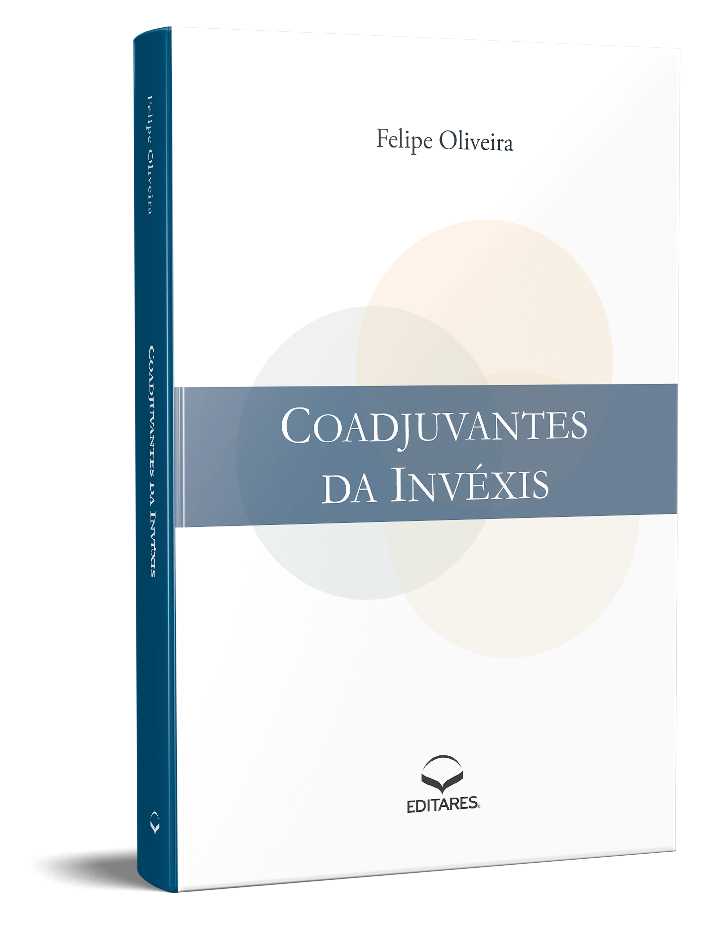
\includegraphics[width=8cm]{articles/entrevista/mockups/Felipe_Oliveira}
\end{center}


\textbf{1. Qual foi a~motivação para a~escrita da obra? Por que a~definição deste tema para publicação de um livro?}

Quando cheguei ao voluntariado da Conscienciologia, em 2013, o~termo amparador extrafísico de função (o primeiro coadjuvante da invéxis) chamou minha atenção. Lembro-me de um voluntário comentar sobre a~importância de se ter livros que abordassem esse tema. Naquele ano, iniciei uma pesquisa para compreender melhor esse conceito e,~em 2014, escrevi meu primeiro artigo de Conscienciologia, apresentado em uma atividade interna do IIPC Ribeirão Preto.

Em 2014, conheci a~técnica da invéxis e~comecei a~estudá-la, iniciando sua aplicação deliberada apenas em 2015. Deparei-me com o~termo Coadjuvantes da Invéxis no tratado 700 Experimentos da Conscienciologia, que, na seção Invexibilidade, apresenta três coadjuvantes fundamentais para a~motivação e~sustentação da invéxis: o~contato mais direto com o~amparo de função, a~fruição da vida intelectual dinamizada e~o~grupo de inversores existenciais (Grinvex). Observando a~convergência desses temas e~motivado pelo interesse em sustentar a~invéxis de modo vitalício, decidi aprofundar minhas pesquisas e~escrever sobre o~assunto. Dessa iniciativa surgiram diversos artigos e~verbetes.

\textbf{2. Quais foram as principais percepções, intra e~extrafísicas, durante a~pesquisa e~a~escrita da obra? E~posterior ao lançamento?}

Ao longo da escrita do livro, tive vários \emph{insights} e~fenômenos parapsíquicos que contribuíram para o~desenvolvimento da obra, desde sugestões telepáticas para inclusão de capítulos até retrocognições marcantes. A~mais significativa ocorreu em 24 de janeiro de 2024, enquanto escrevia o~capítulo Coadjuvante Parapsíquico, que aborda o~amparo de função. Durante esse fenômeno, estava com papel e~pena à~mão, vivenciando um conflito íntimo: acreditava que não deveria escrever sobre parapsiquismo e~a~interação com consciexes, e~que em função disso poderia ser perseguido e~executado. Essa omissão, motivada pela autopreservação, está sendo retratada agora, representando uma retratação com o~passado que começa a~se concretizar.

\textbf{3. Qual o~maior aprendizado com a~escrita desta obra?}

Um dos maiores aprendizados que obtive com a~escrita da obra foi confiar mais nas próprias ideias e~parapercepções. Percebi que havia consciexes interessadas, motivadas e~felizes com a~publicação do livro, o~que me incentivou ainda mais.

\begin{pullquote}
``Percebi que havia consciexes interessadas, motivadas e~felizes com a~publicação do livro, o~que me incentivou ainda mais.''
\end{pullquote}

\textbf{4. O~que poderia dizer como incentivo para que mais pesquisadores invistam na publicação de obras conscienciológicas?}

A escrita de um livro conscienciológico é~desafiadora, pois envolve o~auto e~heterodesassédio consciencial. Cada indivíduo é~uma verdadeira Enciclopédia Consciencial, e~a~publicação de obras sob o~enfoque da Conscienciologia representa uma forma de retribuição ao investimento do Curso Intermissivo em nós, intermissivistas.


\begin{pullquote}
``Cada indivíduo é~uma verdadeira Enciclopédia Consciencial.''
\end{pullquote}

    
    \end{multicols}
\end{document}
